\subsection{Electron}
\label{sec:electron}

Many interesting physical processes are with the involvement of one or more electrons (or positrons) at the LHC.
But these electrons can be subjected to large amount of backgrounds such as hadrons, non-prompt electrons from photon conversions and non-isolated electrons from heavy flavor hadon decays.
It is therefore essential to efficiently reconstruct and identify electrons as well as, in the meantime, to keep high background rejection.

In ATLAS, in central region, the electrons leave tracks in inner detector (ID) and deposit the energies in the electromagnetic (EM) calorimeter. 
Firstly the signals from calorimeter are used for L1 trigger system, and then combined with the information from ID tracks to reconstruct electron candidates that will be used for the high level trigger (HLT) decision algorithms~\cite{ATLAS-CONF-2016-024}.
The backgrounds mentioned above can then be further suppressed by using several identification criteria.
In addition, electrons are required to be isolated from other activities to be further distinguished from background.

More details of electron \textit{reconstruction}, \textit{identification} and \textit{isolation} are described as below.

\textbf{Electron reconstruction} 

Several steps are proceeded for electron reconstruction in the region of $|\eta| < 2.47$ in ATLAS detector:
\begin{enumerate}
	\item \textbf{Seed-cluster reconstruction:} A sliding window of $3 \times 5$ in unit of $\Delta\eta^{tower} \times \Delta\phi^{tower} = 0.025 \times 0.025$ in $\eta \times \phi$ space is utilized to search for electron cluster seeds with total cluster transverse energy greater than 2.5 GeV. Then a clustering algorithm\cite{Lampl:1099735} is applied to form the clusters around the seeds, which can take advantage of removing the duplications. The kinematics of clusters are then reconstructed by using an extended window depending on the cluster position. The efficiency of cluster search is from about $95\%$ at $E_{T} = 7 GeV$ to $99\%$ for $E_{T} \geq 15 GeV$.
	\item \textbf{Track reconstruction:} The track reconstruction can be divided into two steps: pattern recognition and track fit. The standard pattern recognition in ATLAS uses pion hypothesis for energy loss caused by interactions with detector material. If a track seed with $p_{T}$ > 1~\gev~ cannot be successfully extended to a full track required at least seven hits using this pion hypothesis, but still falls inside one of the EM cluster region of interest, as a second attempt, the pattern recognition using electron hypothesis is then used to allow larger energy loss.
Depending on the pattern used in previous stage, the track candidates are then fitted with either the pion hypothesis or the electron hypothesis by using ATLAS Global $\chi^{2}$ Track Fitter\cite{Cornelissen_2008}. If a track candidate fails the fit by using pion hypothesis, it can be refit with the electron hypothesis again. In this method, a specific electron-oriented algorithm is integrated into the ATLAS standard track reconstruction, which improves the performance for electron and as well as maintain minimal interference with the main track reconstruction. 
	\item \textbf{Electron specific track fit:} Once the tracks are obtained, they are loosely matched to EM cluster using the distance in $\eta$ and $\phi$ between the position of track (after extrapolation) in calorimeter's middle layer and the cluster barycentre. The matching conditions take into account the energy loss of bremsstrahlung and the number of precise hits in silicon detector.
	\item \textbf{Electron candidate reconstruction:} The electron candidate is reconstructed by matching the track candidate to EM cluster seed to eventually completes the electron reconstruction procedure. If more than one track satisfy the matching condition, one track is chosen as primary track based on the information of the cluster-track distance R, the number of pixel hits and the presence of a hit in the first silicon layer\cite{ATLAS-CONF-2014-032}.
In addition, the electron candidates are removed from electron pool if it's without any associated precise hit tracks, and moved into photon candidates pool. Then we reformed the electron clusters by using $3 \times 7$ ($5 \times 5$) longitudinal towers of cells in barrel (end-caps) in EM calorimeter. The measured energy is calibrated to original electron energy based on MC simulated samples by using multivariate techniques (MVA).
\end{enumerate}

In addition, in physics analysis, to reduce the background from photon conversions and secondary particles, the track associated with electron is required to be compatible with the primary vertex of the hard collision. 
Practically, the impact parameters cuts such as $d_{0}/\sigma_{d_{0}} < 5$ and $z_{0}sin\theta$ < 0.5 mm are usually applied, where $d_{0}$ is the closest distance of the track to the measured beam-line, $z_{0}$ is the distance along the beam-line between the point where $d_{0}$ is measured and the beam-spot position, and $\theta$ is polar angle of the track, $\sigma_{d_{0}}$ denotes the estimated uncertainty of $d_{0}$ parameter. 
Figure~\ref{fig:ele_d0z0} depicts the definition of each track impact parameter.
\begin{figure}[!htb]
  \centering
  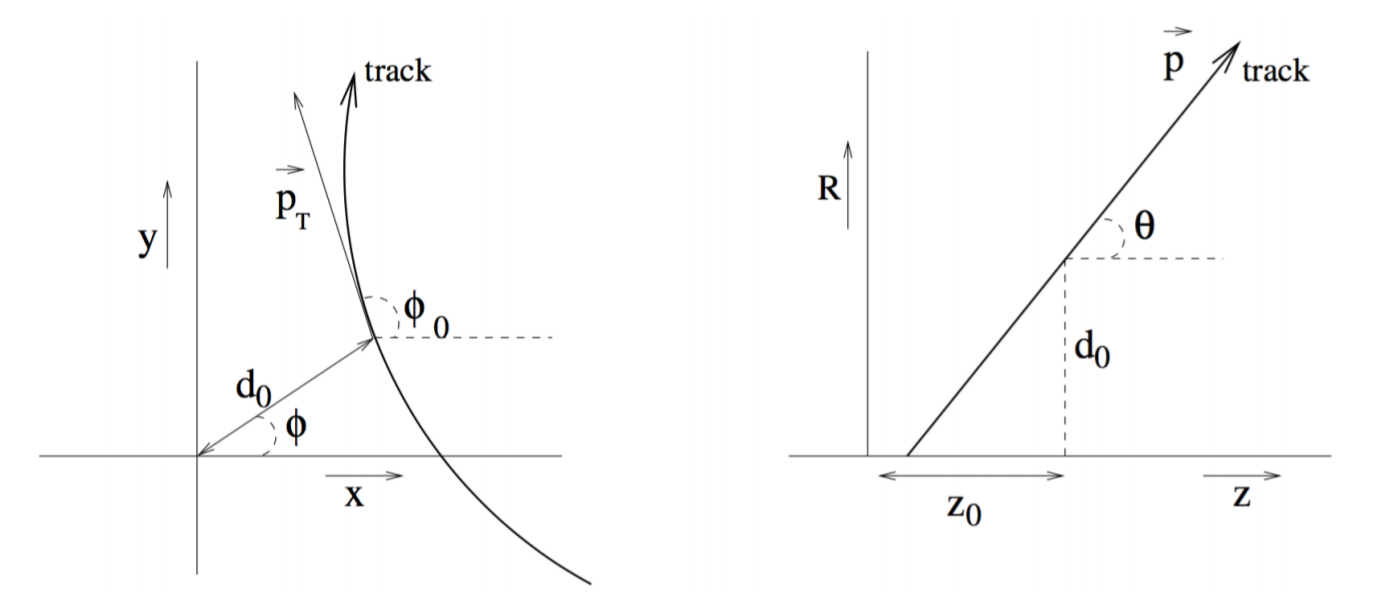
\includegraphics[width=0.9\textwidth]{figures/Simulation/track_parameter_2d.png}
  \caption{Schematic of the impact parameters of a track in the transverse plane (left)
and RZ-plane (right), as defined in the global ATLAS tracking frame\cite{Limper:1202457}.}
  \label{fig:ele_d0z0}
\end{figure}

\textbf{Electron identification}

The electron identifications are applied to determine whether the reconstructed electron candidate is more signal-like or background-like object.
The identification algorithms make use of quantities of related variables from electron cluster and track measurements including calorimeter shower shapes, track properties, 
as well as variables measuring bremsstrahlung effects for distinguishing signal from background.
Taking the advantage of new IBL in run-2, the number of hits in this innermost pixel layer is utilized for discriminating between electrons and converted photons.
In addition, a likelihood method based on the TRT high-threshold hits is adopted to compensate the lower transition radiation absorption probability of the argon.

The baseline identification algorithm introduced in ATLAS run-2 is the likelihood-based (LH) method, making use of a MVA technique to simultaneously evaluate several properties of electron candidates when making a decision.
The LH method utilizes the probability density functions (PDFs) of signal and background as the input discriminating variables.
Based on these PDFs, it can calculate overall probabilities of the object to be signal or background.
Then the probabilities of signal and background are combined together into a discriminant $d_{\mathcal{L}}$:
\begin{equation}
	d_{\mathcal{L}} = \frac{\mathcal{L}_{S}}{\mathcal{L}_{S} + \mathcal{L}_{B}},
	~~ \mathcal{L}_{S(B)}(\vec{x}) = \prod_{i=1}^{n} P_{s(b),i}(x_{i})	
\end{equation}
where $\vec{x}$ denotes the vector of discriminating variables and $P_{s(b),i}(x_{i})$ represents the value of signal (background) PDF of the $i^{th}$ varaible as $x_{i}$.

Three levels of working points (WPs) for electron identification are provided: \textit{Loose}, \textit{Medium} and \textit{Tight}, in order of incresing background rejection.
Samples selected by a looser WP are subsets of a tighter one, for example, the electrons passing Medium can all be selected by Loose.
The identification efficiency varies as function of transverse energy ($E_{T}$) as shown in figure~\ref{fig:ele_IDeff}.
For evaluations, the electron candidates from MC simulation of $Z \rightarrow ee$ decays (di-jet) are used as signal (background).
Depending on the working point, the signal (background) efficiencies for reconstructed electron candidates at $E_{T} = 25 GeV$ are from 78 to 90\% (0.3 to 0.8\%), and increase (decrease) with $E_{T}$.
\begin{figure}[!htb]
  \centering
  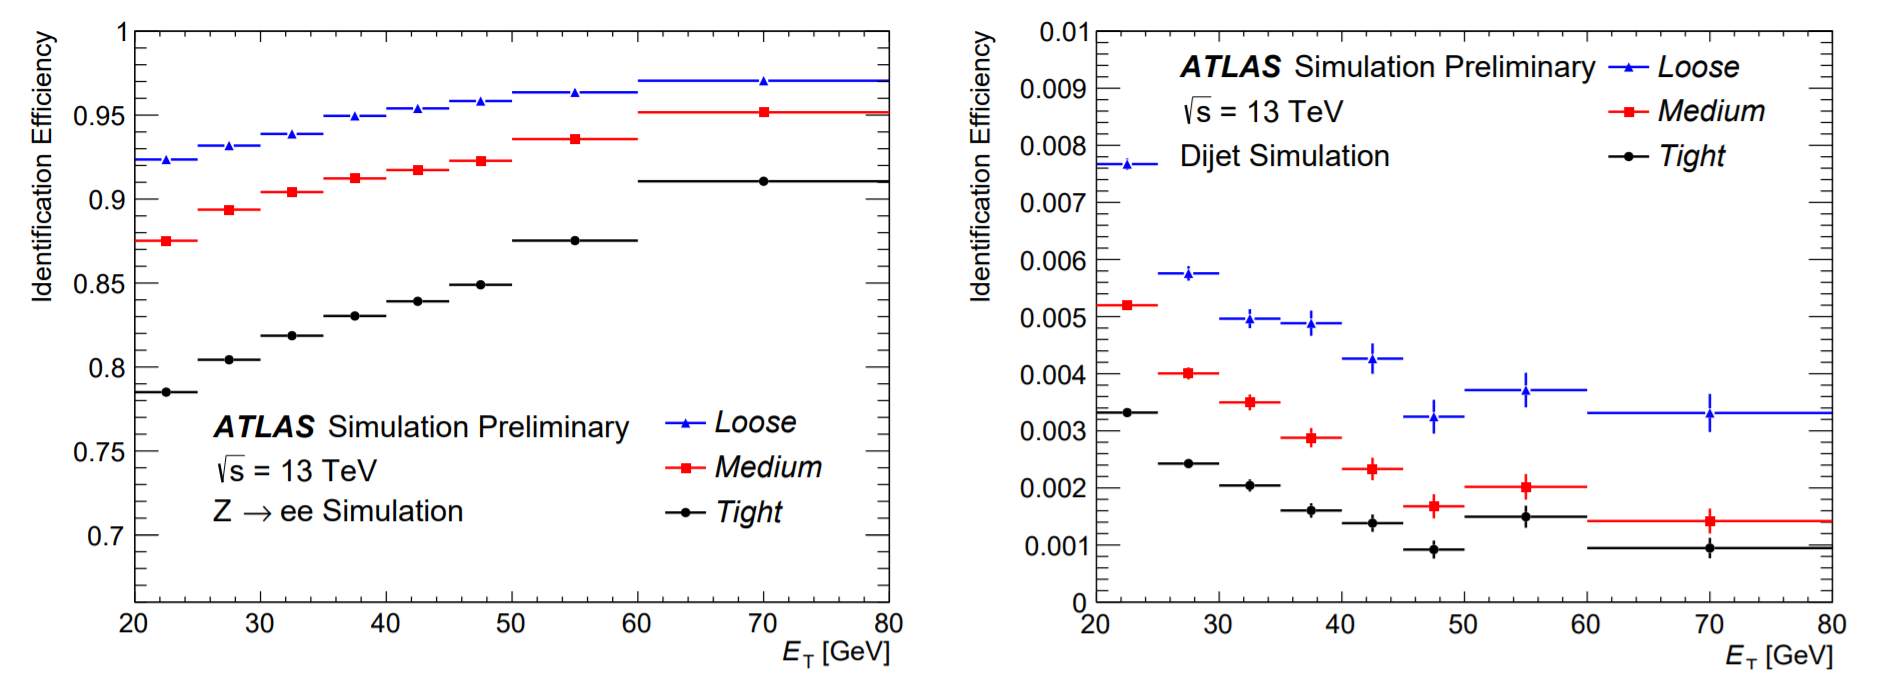
\includegraphics[width=0.9\textwidth]{figures/Simulation/ele_id_eff.png}
  \caption{The efficiencies of three electron identification WPs from $Z \rightarrow ee$ (left) events and hadrons misidentified as electrons estimated using di-jet MC samples (right).}
  \label{fig:ele_IDeff}
\end{figure}

\textbf{Electron isolation}

In addition to the identification criteria, most analyses have electron isolation requirement to further distinguish signal from background.
To quantify the energy of particles around the electron candidate, the isolation variables can help to separate the prompt electron from other non-isolated electrons, like the electrons from converted photons or from heavy flavour hadron decays.
There are two kinds of discriminating variables that have been designed:
\begin{itemize}
	\item \textbf{Calorimeter-based variable:} $E_{T}^{topocone20}$. 
        It's computed from the sum of transverse energies of topological clusters~\cite{Aad:2016upy}, and calibrated at EM scale in a cone of $\Delta R = 0.2$ around the candidate electron cluster. 
        It only considers the clusters with positive reconstructed energy. In addition, a correction as a function of $(E_{T}, \eta)$ values is applied to account for the electron energy leakage outside the cluster.
	\item \textbf{Track-based variable:} $p_{T}^{varcone20}$. It's calculated as the sum of transverse momentum of all satisfied tracks within a cone of $\Delta R = min(0.2, 10 GeV/E_{T})$ around the candidate electron track. To calculate the sum, it requires the tracks are originating from the reconstruction PV of hard collision, and exclude the associated tracks of electron itself.
\end{itemize}
Based on the values of $E_{T}^{topocone20}/p_{T}$ and $p_{T}^{varcone20}/p_{T}$, a serious of working points with different selection requirements are defined.
The resulting WPs are divided into two kinds:
\begin{itemize}
	\item Efficiency targeted working points: varying requirements to obtain a certain isolation efficiency, which can either be a constant or as a function of $E_{T}$.
	\item Fixed requirement working points: set the constant upper thresholds on isolation variables.
\end{itemize}
The distribution of two discriminating variables are shown in figure~\ref{fig:ele_iso} for $ZZ \rightarrow ee$ events with $E_{T} > 27 GeV$ and satisfying \textit{Tight} requirement.
\begin{figure}[!htb]
  \centering
  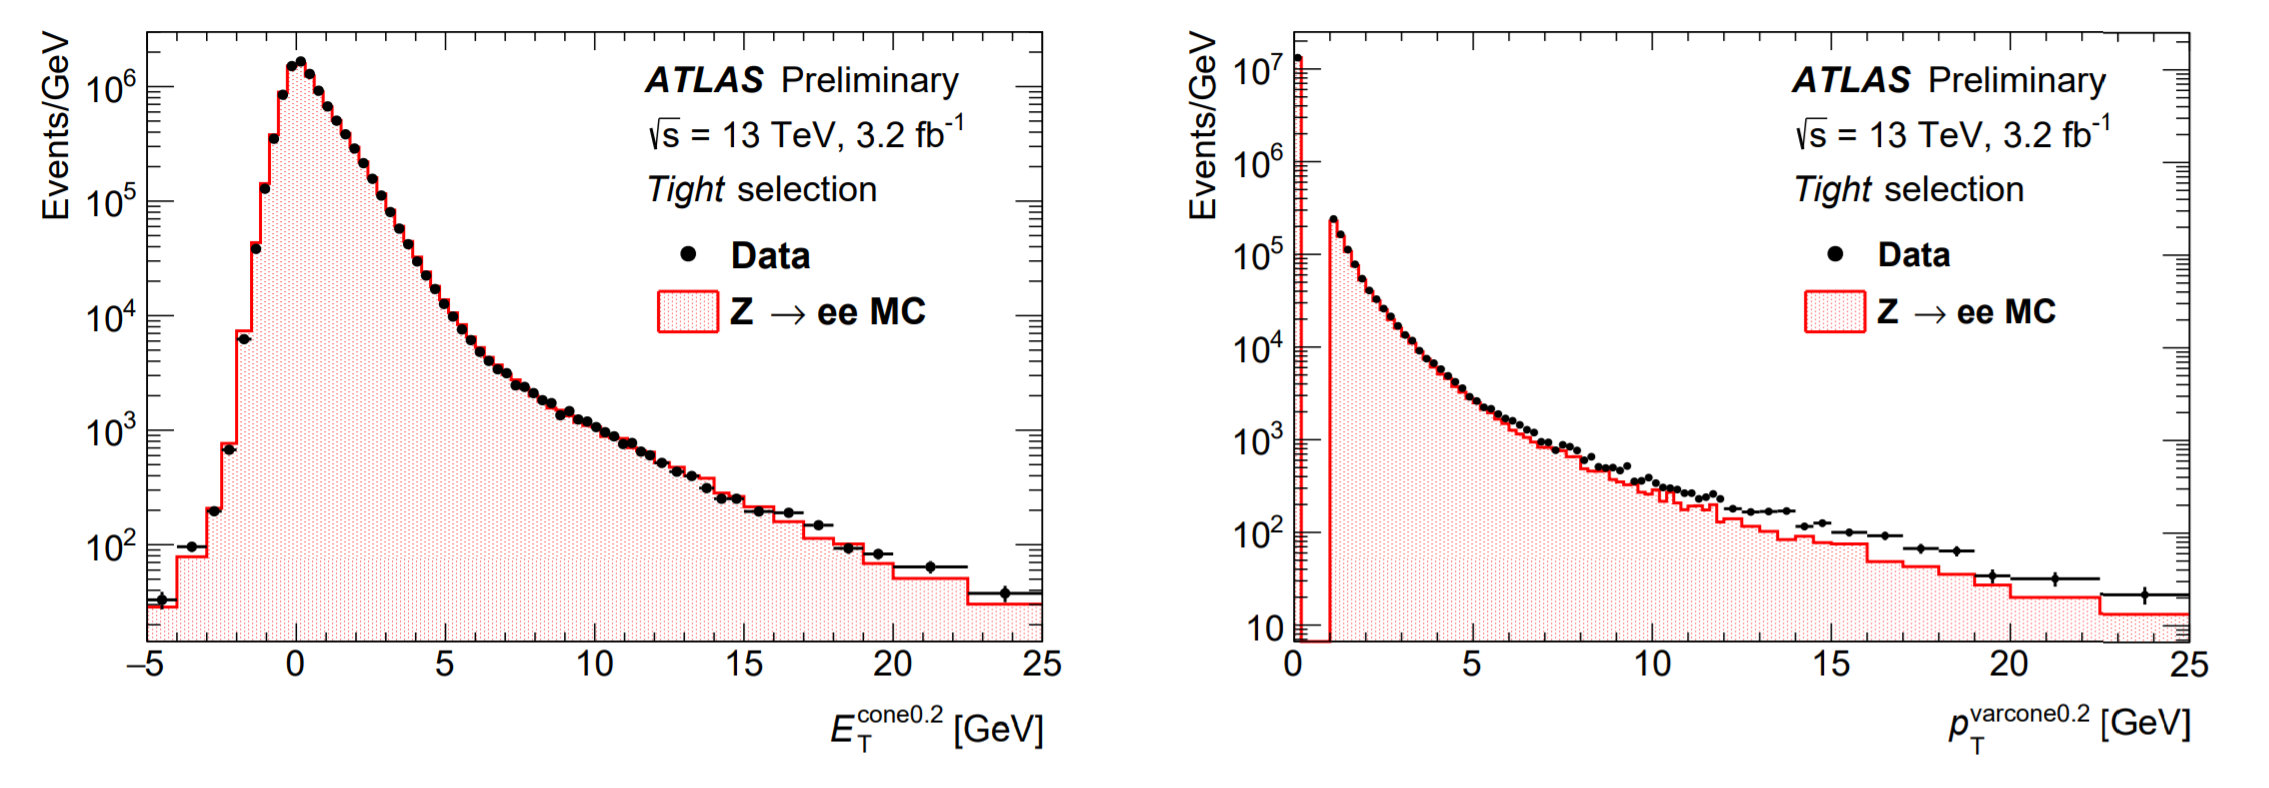
\includegraphics[width=0.9\textwidth]{figures/Simulation/ele_iso.png}
  \caption{$E_{T}^{cone0.2}$ (left) and $p_{T}^{varcone0.2}$ (right) distribution for electrons from $ZZ \rightarrow ee$ events in data and MC simulation. The simulated events (full histograms) are normalized to data.}
  \label{fig:ele_iso}
\end{figure}

